%%%%%%%%%%%%%%%%%%%%%%%%%%%%%%%%%%%%%%%%%%%%%%%%%%%%%%%%%%%%%%%%%%%%%%%%%%%%%%
% Customisable conference poster template with BioMedIA logo and Imperial
% colour style.
%
% Adapted from Kevin Keraudren's template from the internal BioMedIA pages
% and from baposter/examples/ECCS2011/poster.tex
%
% Author: Christian Baumgartner (c.f.baumgartner@gmail.com)
% Date: 11. October 2016
%

% add "debug" as option for debugging output
\documentclass[paperwidth=841mm,paperheight=1300mm,portrait]{baposter}

\usepackage{relsize}                  % For \smaller
\usepackage{url}                      % For \url
\usepackage{epstopdf}                 % Included EPS files automatically converted to PDF to
                                      % include  with pdflatex

\usepackage{multicol}                 % multiple columns
\usepackage[superscript,nomove]{cite} % for superscript citing

\usepackage{enumitem}                 % to change leftmargin of bullet lists
\usepackage{booktabs}                 % nicer tables

\usepackage{tikz}                     % To draw background
\usepackage{amsmath,amssymb,enumerate}
\usepackage{subfigure}
\usepackage{caption}
\usepackage{graphicx}

%%% Global Settings %%%%%%%%%%%%%%%%%%%%%%%%%%%%%%%%%%%%%%%%%%%%%%%%%%%%%%%%%%%

\graphicspath{{figures/}}            % Root directory of the pictures
\tracingstats=2                      % Enabled LaTeX logging with conditionals

%%% Color Definitions %%%%%%%%%%%%%%%%%%%%%%%%%%%%%%%%%%%%%%%%%%%%%%%%%%%%%%%%%

% Those are the official imperial colours:
\definecolor{Navy}{RGB}{0,33,71}
\definecolor{ImperialBlue}{RGB}{0,62,116}
%\definecolor{LightGrey}{RGB}{255,250,250}
\definecolor{LightGrey}{RGB}{255,254,254}
%\definecolor{CoolGrey}{RGB}{157,157,157}
\definecolor{LightBlue}{RGB}{212,239,252}
\definecolor{Black}{RGB}{0,0,0}
\definecolor{White}{RGB}{248,250,252}
%\definecolor{LightGrey}{RGB}{248,248,248}


%%%%%%%%%%%%%%%%%%%%%%%%%%%%%%%%%%%%%%%%%%%%%%%%%%%%%%%%%%%%%%%%%%%%%%%%%%%%%%%%
%%% Utility functions %%%%%%%%%%%%%%%%%%%%%%%%%%%%%%%%%%%%%%%%%%%%%%%%%%%%%%%%%%

%%% Save space in lists. Use this after the opening of the list %%%%%%%%%%%%%%%%
\newcommand{\compresslist}{
  \setlength{\itemsep}{3pt}
  \setlength{\parskip}{2pt}
  \setlength{\parsep}{2pt}

\vspace{-0.75em}

}

\newcommand{\tab}{\hspace{0.5em}}

%%%%%%%%%%%%%%%%%%%%%%%%%%%%%%%%%%%%%%%%%%%%%%%%%%%%%%%%%%%%%%%%%%%%%%%%%%%%%%%
%%% Document Start %%%%%%%%%%%%%%%%%%%%%%%%%%%%%%%%%%%%%%%%%%%%%%%%%%%%%%%%%%%%
%%%%%%%%%%%%%%%%%%%%%%%%%%%%%%%%%%%%%%%%%%%%%%%%%%%%%%%%%%%%%%%%%%%%%%%%%%%%%%%

\begin{document}
\typeout{Poster rendering started}
\sffamily
%%% Setting Background Image %%%%%%%%%%%%%%%%%%%%%%%%%%%%%%%%%%%%%%%%%%%%%%%%%%

\background{
  % Change colours of body background and header background if desired
  % you can also use tikz to include a custom picture here
  \begin{tikzpicture}[remember picture,overlay]%
    %the poster background colour
    \fill[fill=LightGrey] (current page.north west) rectangle (current page.south east);
    %the header
    \fill [fill=LightGrey] (current page.north west) rectangle ([yshift=-\headerheight] current page.north east);
  \end{tikzpicture}
}

%%%   General Poster Settings %%%%%%%%%%%%%%%%%%%%%%%%%%%%%%%%%%%%%%%%%%%%%%%%%%%
%%%%%%   Eye Catcher, Title, Authors and University Images %%%%%%%%%%%%%%%%%%%%%%

\begin{poster}{
  grid=false,
  eyecatcher=true,
  borderColor=White,
  headerColorOne=ImperialBlue,
  headerColorTwo=ImperialBlue,
  headerFontColor=LightGrey,
  boxColorOne=White,
  headershape=roundedright,
  textborder=roundedleft,
  background=user,
  headerborder=none,
  textborder=none,
  boxshade=plain
}
%%% Logo %%%%%%%%%%%%%%%%%%%%%%%%%%%%%%%%%%%%%%%%%%%%%%%%%%%%%%%%%%%%%%%
{
    
\includegraphics[width=0.3\textwidth]{logos/Imperial_logo}
}
%%% Title %%%%%%%%%%%%%%%%%%%%%%%%%%%%%%%%%%%%%%%%%%%%%%%%%%%%%%%%%%%%%%%%%%%%%
{
  {\sf\bf \vspace{2pt} \\
  \textcolor{Black}{RIS-aided Dual-Functional Radar and \\\vspace{4pt}
   Communications Beamforming Design}}
  % move authors list down a little bit
}
%%% Authors %%%%%%%%%%%%%%%%%%%%%%%%%%%%%%%%%%%%%%%%%%%%%%%%%%%%%%%%%%%%%%%%%%%
{ 
  \vspace{5pt}
  \textcolor{Black}{\textit{Author:} Zhaolin Wang \quad \textit{Supervisor:} Prof Bruno Clerckx}
%   \textcolor{Black}{\small $^1$School of Electronic Information, Wuhan University, Wuhan, China}
}

%%%%%%%%%%%%%%%%%%%%%%%%%%%%%%%%%%%%%%%%%%%%%%%%%%%%%%%%%%%%%%%%%%%%%%%%%%%%%%%
%%% Boxes Start %%%%%%%%%%%%%%%%%%%%%%%%%%%%%%%%%%%%%%%%%%%%%%%%%%%%%%%%%%%%%%%
%%%%%%%%%%%%%%%%%%%%%%%%%%%%%%%%%%%%%%%%%%%%%%%%%%%%%%%%%%%%%%%%%%%%%%%%%%%%%%%

%%% Motivation %%%%%%%%%%%%%%%%%%%%%%%%%%%%%%%%%%%%%%%%%%%%%%%%%%%%%%%%%%%%%%%%
\headerbox{Motivation}{name=motivation,column=0,span=1,row=0}{
\small
    \begin{itemize}[leftmargin=1.4em]
        \item \textbf{CRSS}
        \vspace{-4pt}
        \begin{itemize}[leftmargin=1em]
        \vspace{-2pt}\item[$\blacktriangleright$]  Enable two systems perform in the same frequency band with tiny performance loss.
        \vspace{-2pt}\item[$\blacktriangleright$]  Long-term solution for the spectrum management of communications and radar.
        \end{itemize}

        \vspace{-5pt}
        \item \textbf{RIS}
        \vspace{-4pt}
        \begin{itemize}[leftmargin=1em]
        \vspace{-2pt}\item[$\blacktriangleright$]  Modify wireless channel via passive beamforming.
        \vspace{-2pt}\item[$\blacktriangleright$]  Provide extra capability for the CRSS system.
        \end{itemize}

        \vspace{-5pt}
        \item \textbf{Group/fully connected RIS}
        \vspace{-4pt}
        \begin{itemize}[leftmargin=1em]
        \vspace{-2pt}\item[$\blacktriangleright$]  A novel RIS model wherein elements are connected mutually.
        \vspace{-2pt}\item[$\blacktriangleright$]  Lead to higher received power than single connected RIS in Rayleigh channel.
        \end{itemize}

        \item \textbf{WSR maximization}
        \vspace{-4pt}
        \begin{itemize}[leftmargin=1em]
        \vspace{-2pt}\item[$\blacktriangleright$]  The most representative communication metric.
        \item[$\blacktriangleright$]  Has not been investigated in this field.
        \end{itemize}
    \end{itemize}

}

%%% Contribution %%%%%%%%%%%%%%%%%%%%%%%%%%%%%%%%%%%%%%%%%%%%%%%%%%%%%%%%%%%%%%%%%%
\headerbox{Contribution}{name=contribution, column=1,span=1, row = 0, bottomaligned=motivation}{
\small {The \textit{first} work that studies \textbf{WSR} maximization and \textbf{group/fully connected RIS} in CRSS.} \\
\vspace{-6pt}
\begin{itemize}[leftmargin=1.4em]
    \vspace{-4pt}
     \item \textbf{A new framework}
     \begin{itemize}[leftmargin=1.2em]
        \vspace{-6pt}\item[$\blacktriangleright$] A BS with separated or shared deployment probing one target and serving multiple users.
        \vspace{-4pt}\item[$\blacktriangleright$] The users receive signal from BS plus reflected signal from RIS.
     \end{itemize}
    \vspace{-4pt}
    \item \textbf{An AO algorithm for separated deployment}
    \begin{itemize}[leftmargin=1.2em]
        \vspace{-6pt}\item[$\blacktriangleright$] Non-convexity from WSR is tackled by WMMSE framework and Fractional Programming (FP).
        \vspace{-4pt}\item[$\blacktriangleright$] Non-convexity from group connected RIS is tackled by scattering-reactance relationship.
    \end{itemize}
    \vspace{-4pt}
    \item \textbf{An AO algorithm for shared deployment}
    \begin{itemize}[leftmargin=1.2em]
        \vspace{-6pt}\item[$\blacktriangleright$] Similar as separated deployment, but additional non-convexity from radar constant-modulus constraint.
        \vspace{-6pt}\item[$\blacktriangleright$] Lower complexity SDR method than the existing Majorization-Minimization (MM) method.
    \end{itemize}
\end{itemize}
}

%%% System setup %%%%%%%%%%%%%%%%%%%%%%%%%%%%%%%%%%%%%%%%%%%%%%%%%%%%%%%%%%%%%%%%%%%%
\headerbox{Separated/Shared Setup}{name=setup, column=2, span=1, row = 0, bottomaligned=contribution}{
\vspace{10pt}
\begin{minipage}[c]{\textwidth}
    \centering
    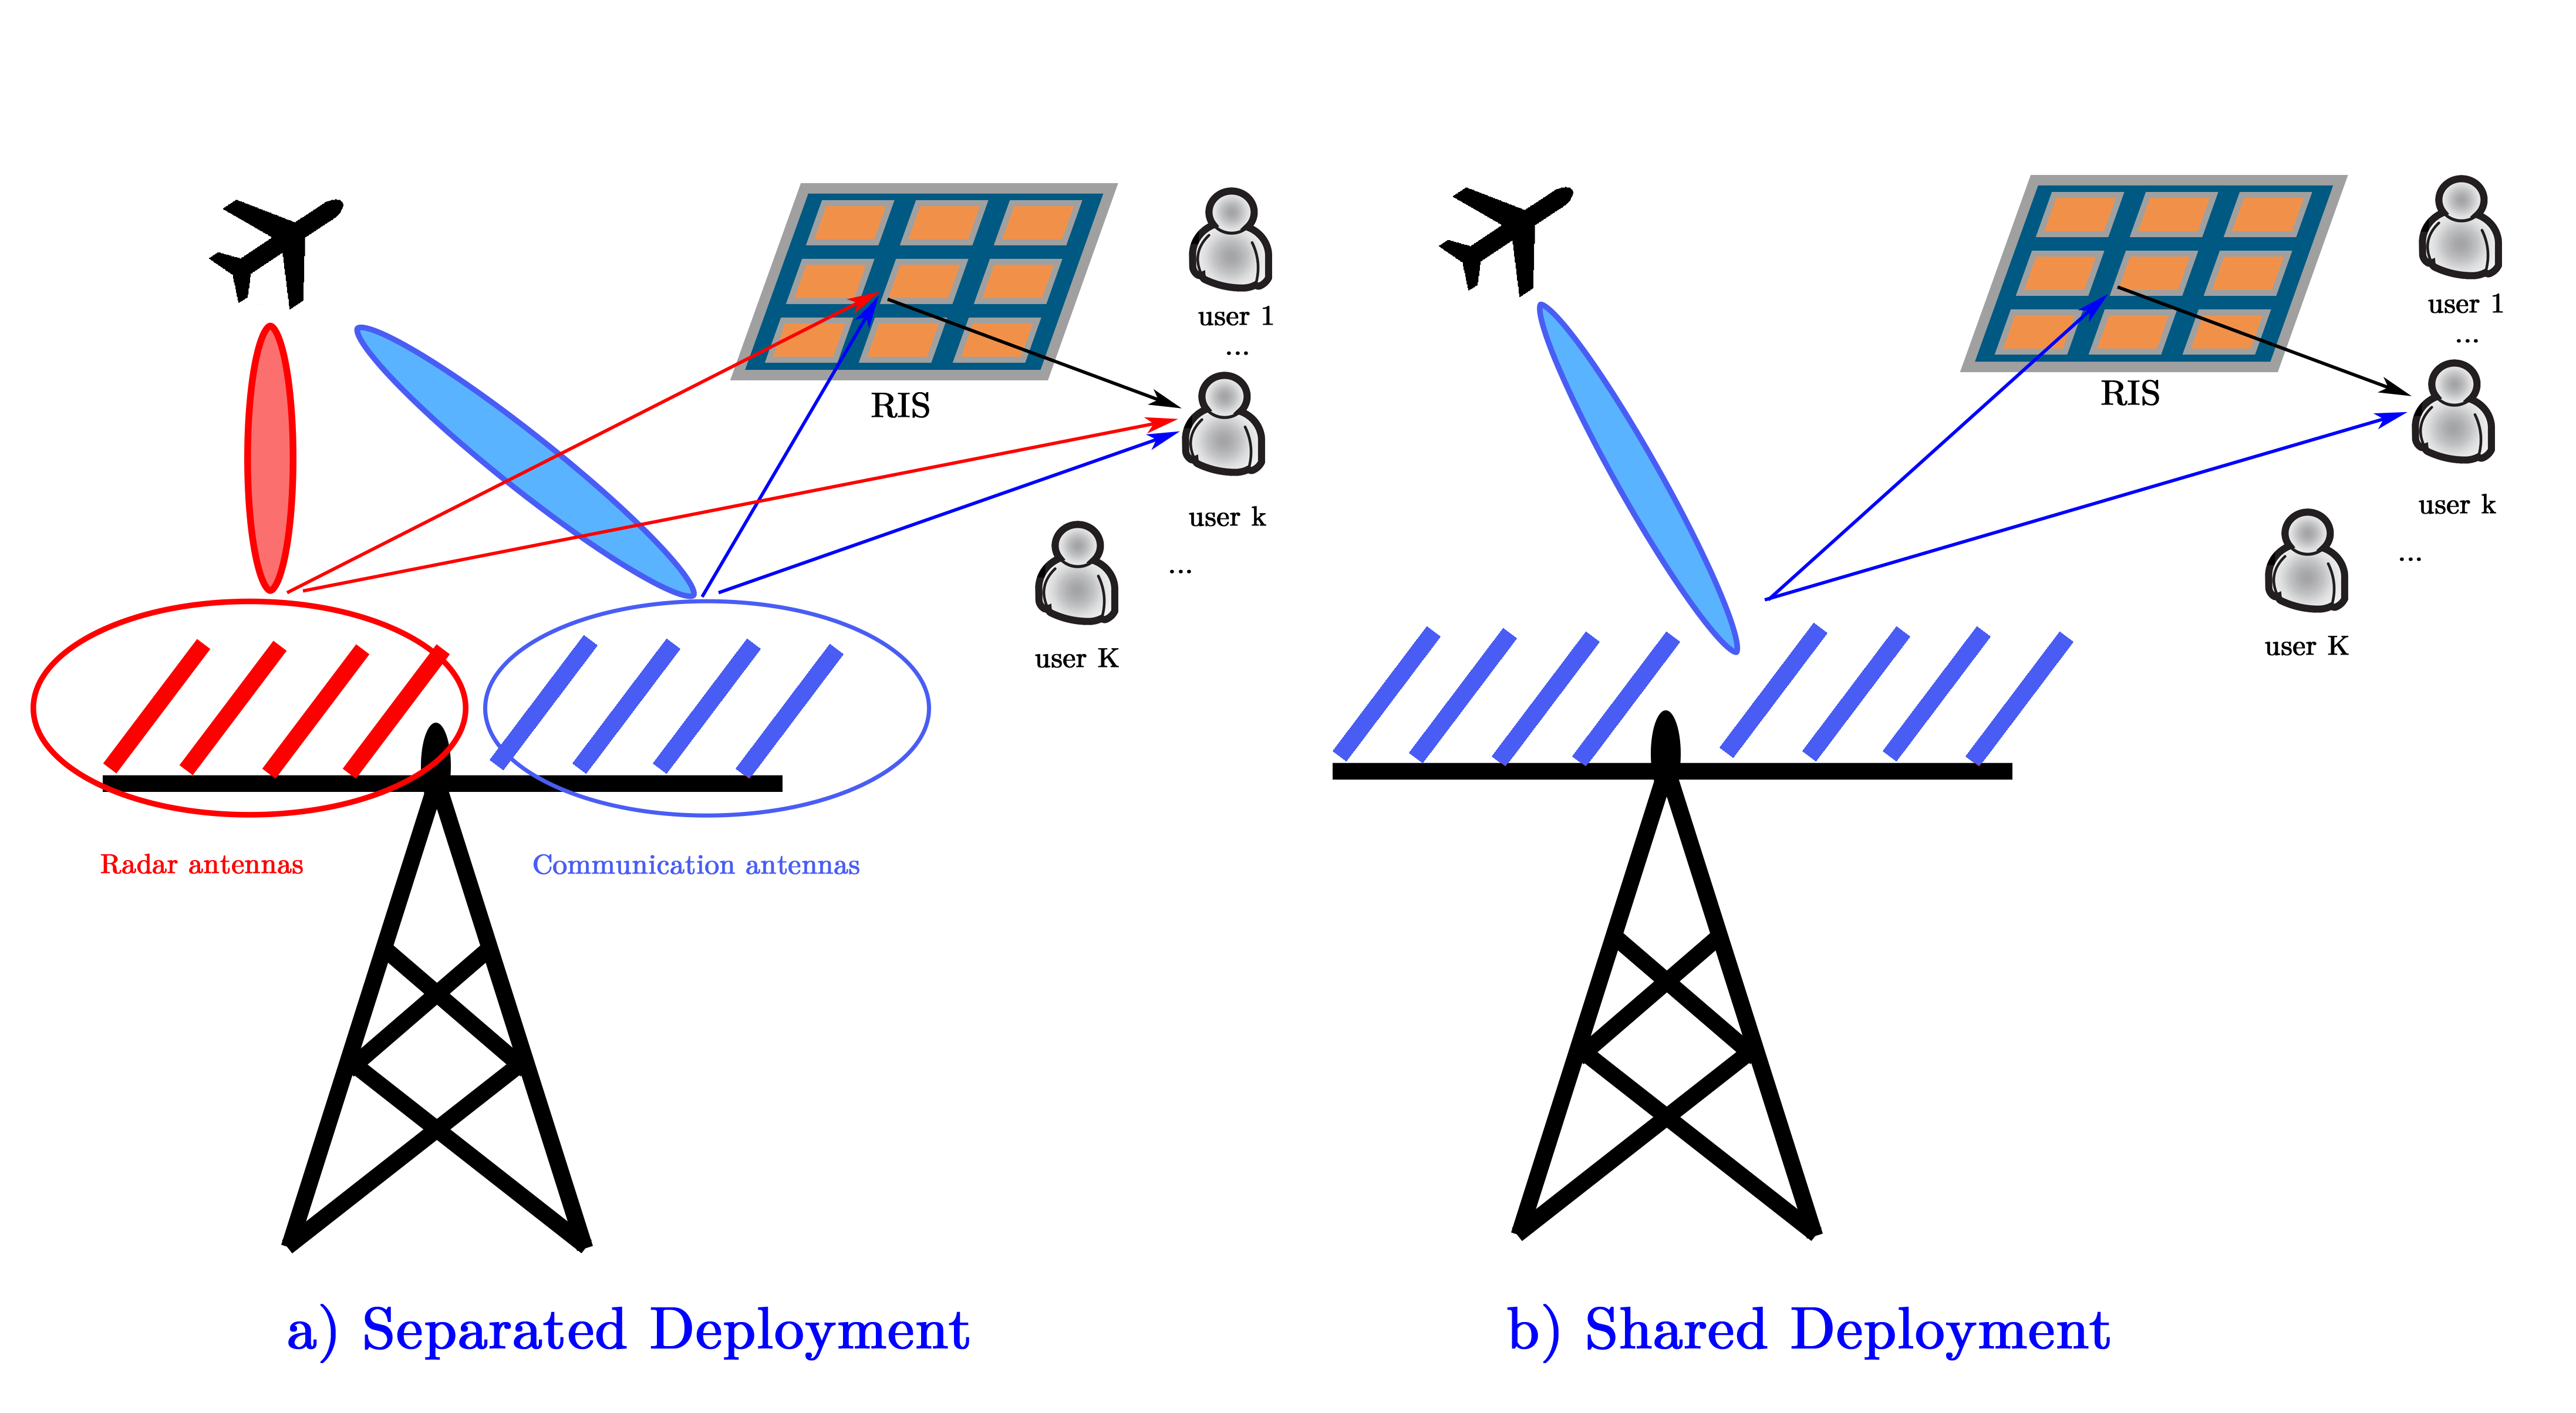
\includegraphics[width=1.0\textwidth]{fig/setup}
\end{minipage}\\
 \vspace{-8pt}
\begin{itemize}[leftmargin=1 em]
\small{
\item Separated: two groups of antennas transmit radar and communication signals separately. \vspace{-6pt}
\item Shared: all antennas transmit communication signal under radar constraint.\vspace{-6pt}
\item Tradeoff between complexity and performance.
}
\end{itemize}
}

%%% System model %%%%%%%%%%%%%%%%%%%%%%%%%%%%%%%%%%%%%%%%%%%%%%%%%%%%%%%%%%%%%%%%%%%%
\headerbox{System Model}{name=model, column=0, span=1, below=motivation}{
\begin{minipage}[c]{\textwidth}
\small
\begin{itemize}[leftmargin=1.4 em]
 \vspace{-2pt}
\item \textbf{Separated}: received signal at user $k$
\vspace{-4pt}
\begin{align}\notag
    y_k &= (\mathbf{h}_k^H \mathbf{\Theta}^H \mathbf{H}_c + {\bf d}_{c,k}^H) \sum_{j=1}^K \mathbf{p}_j s_j \\
    &+ (\mathbf{h}_k^H \mathbf{\Theta}^H \mathbf{H}_r + {\bf d}_{r,k}^H) \mathbf{q} + n_k \nonumber
\end{align}
${\blacktriangleright}$ $s_j$: data symbol; ${\bf p}_j$: linear precoder; ${\bf q}$: radar signal; ${\bf d}_{c,k}, {\bf d}_{r,k}$: direct channel;
${\bf H}_c, {\bf H}_r$: BS $\rightarrow$ RIS channel; ${\bf h}_k$: RIS $\rightarrow$ user channel; ${\bf \Theta}$: passive beamforming matrix.

\vspace{-2pt}
\item \textbf{Shared}: received signal at user $k$
\vspace{-4pt}
\begin{equation}\notag
    \check{y}_k = ({\bf h}_k^H {\bf \Theta}^H {\bf H} + {\bf d}_k^H) \sum_{j=1}^K \check{\bf p}_j s_j
\end{equation}
${\blacktriangleright}$ $s_j$: data symbol; $\check{\bf p}_j$: linear precoder; ${\bf d}_{k}$: direct channel;
${\bf H}$: BS $\rightarrow$ RIS channel; ${\bf h}_k$: RIS $\rightarrow$ user channel; ${\bf \Theta}$: passive beamforming matrix.
\small

\item \textbf{WSR}: $R = \sum_{k=1}^K \mu_k \log_2(1+\mathrm{SINR}_k)$
\item \textbf{Probing power}: $d(\varphi_m) = {\bf{a}}^H(\varphi_m) {\bf{C}} {\bf{a}}(\varphi_m)$ with ${\bf a}(\varphi_m)$ denoting steering vector and ${\bf C}$ denoting covariance matrix of overall transmit signal.
\item \textbf{Radar constant-modulus constraint}:\\
${\blacktriangleright}$ power fed to each antenna is the same.
\begin{align*}
    &\text{Separated:} \quad \mathrm{diag}(\mathbf{R}_{\bf q}) = \frac{P_r}{M_r}\mathbf{1}^{M_r \times 1}\\
    &\text{Shared:} \quad \mathrm{diag}\left( \sum_{k=1}^K \check{\bf p}_k \check{\bf p}_k^H \right) = \frac{P}{M}{\bf 1}^{M \times 1}
\end{align*}
\end{itemize}
\end{minipage}
}

%%% Algorithm %%%%%%%%%%%%%%%%%%%%%%%%%%%%%%%%%%%%%%%%%%%%%%%%%%%%%%%%%%%%%%%%%%%
\headerbox{Algorithm for WSR and Probing Power Maximization}{name=algorithm, column=1,span=2, below=motivation, bottomaligned = model}{
\small
\emph{1)} \textbf{WMMSE: fix passive beamforming, optimize active beamforming}
    \begin{itemize}
        \vspace{-2pt}\item[$\blacktriangleright$] Calculate MMSE receiver for each user $k$ as $g_k^{\mathrm{MMSE}} = \arg \min_{g_k} \mathbb{E} \left[ \Vert g_ky_k - s_k \Vert^2 \right]$
        \vspace{-2pt}\item[$\blacktriangleright$] According WMMSE to framework, the WSR maximization w.r.t. active beamforming can be converted to weighted MSE minimization problem with MMSE receiver.

        \begin{equation}\notag
            \max_{{\bf p}_k, {\bf R_q} \in \mathcal{F}} \overbrace{\sum_{k=1}^K \mu_k \log_2(1+\mathrm{SINR}_k)}^{\text{non-convex}} \quad  \Longrightarrow \min_{{\bf p}_k, {\bf R_q} \in \mathcal{F}} \overbrace{\sum_{k=1}^K w_k \mathbb{E} \left[ \left\Vert g_k^{\mathrm{MMSE}}y_k - s_k \right\Vert^2 \right]}^{\text{convex}}
        \end{equation}
        \begin{minipage}[c]{\textwidth/3}
                $\blacksquare$ Separated
                \begin{itemize}
                    \vspace{-2pt}\item[$\bullet$] Feasible set $\mathcal{F}$ is convex.
                    \vspace{-2pt}\item[$\bullet$] directly solved using CVX toolbox.
                \end{itemize}   
  
        \end{minipage}
        \begin{minipage}[c]{\textwidth/2}
                $\blacksquare$ Shared
                \begin{itemize}
                    \vspace{-2pt}\item[$\bullet$] Feasible set $\mathcal{F}$ is non-convex.
                    \vspace{-2pt}\item[$\bullet$] using SDR technique and dominant eigenvalue approximation.
                \end{itemize}  
        \end{minipage}
    \end{itemize}
\vspace{2pt}
\emph{2)} \textbf{FP: fix active beamforming, optimize passive beamforming}
    \begin{itemize}
        \vspace{-2pt}\item[$\blacktriangleright$] Based on FP, the WSR maximization w.r.t. passive beamforming can be reformulated as a minimization problem with a convex objective function through \textit{Lagrangian dual transform} and \textit{quadratic transform}.
        \begin{equation}\notag
            \max_{{\bf \Theta} \in \mathcal{Q}} \overbrace{\sum_{k=1}^K \mu_k \log_2(1+\mathrm{SINR}_k)}^{\text{non-convex}} \quad \Longrightarrow \min_{\stackrel{\boldsymbol{\theta} = \mathrm{vec}({\bf \Theta}^H)}{{\bf \Theta} \in \mathcal{Q}}} \overbrace{\boldsymbol{\theta}^H {\bf U} \boldsymbol{\theta} - 2 \mathrm{Re} \left\{ \boldsymbol{\theta}^H {\bf v} \right\}}^{\text{convex}}
        \end{equation}
        \begin{minipage}[c]{\textwidth/3}
            $\blacksquare$ Single connected RIS
            \begin{itemize}
                \vspace{-2pt}\item[$\bullet$] Feasible set $\mathcal{Q}$ is convex.
                \vspace{-2pt}\item[$\bullet$] directly solved using CVX toolbox.
            \end{itemize}   
        
        \end{minipage}
        \begin{minipage}[c]{\textwidth/2}
                $\blacksquare$ Group/fully connected RIS
                \begin{itemize}
                    \vspace{-2pt}\item[$\bullet$] Feasible set $\mathcal{Q}$ is non-convex.
                    \vspace{-2pt}\item[$\bullet$] using scattering-reactance relationship to formulate an equivalent unconstrained problem, which can be addressed by Quasi-Newton method.
                \end{itemize}  
        \end{minipage}
    \end{itemize}

\vspace{-2pt}
\emph{3)} \textbf{Alternating between \emph{1)} and \emph{2)} until convergence}
}


%%% Beampattern %%%%%%%%%%%%%%%%%%%%%%%%%%%%%%%%%%%%%%%%%%%%%%%%%%%%%%%%%%%%%%%%
\headerbox{Beampattern Comparison}{name=beampattern, column=0,span=2, below=algorithm, above=bottom}{

    \begin{minipage}[c]{0.26\textwidth}
        % \vspace{-200pt}
        $\blacktriangleright$ In both separated and shared deployments, the RIS aids the system in achieving
        improved radar beampatterns.
        \vspace{5pt}\\
        $\blacktriangleright$ The fully connected RIS brings more improvements in terms of radar beampattern
        and achievable region than single connected RIS in Rayleigh channel,
        while its performance is the same as single connected RIS in LOS channel.
        \vspace{5pt}\\
        $\blacktriangleright$ Compared with separated deployment, the shared deployment achieves better beampattern because the antennas are fully exploited.
    \end{minipage}
    \begin{minipage}[c]{0.37\textwidth}
        \vspace{10pt}
        \begin{minipage}[c]{\textwidth}
            \centering
            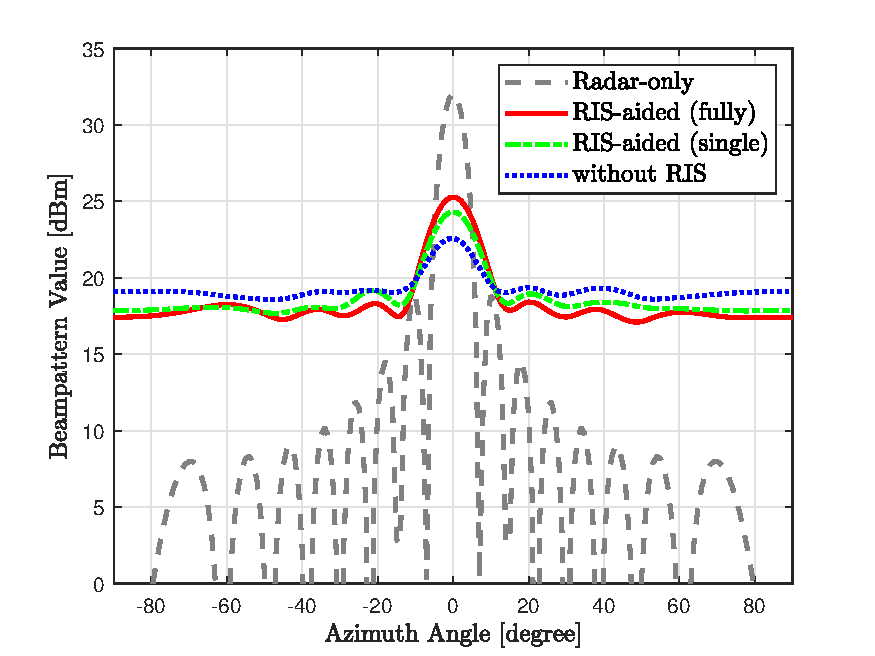
\includegraphics[width=0.95\textwidth]{fig/beampattern_rayleigh_single_fully_b}\vspace{2pt}\\
            \small{a) Separated, Rayleigh}
        \end{minipage}\vspace{10pt}\\
        \begin{minipage}[c]{\textwidth}
            \centering
            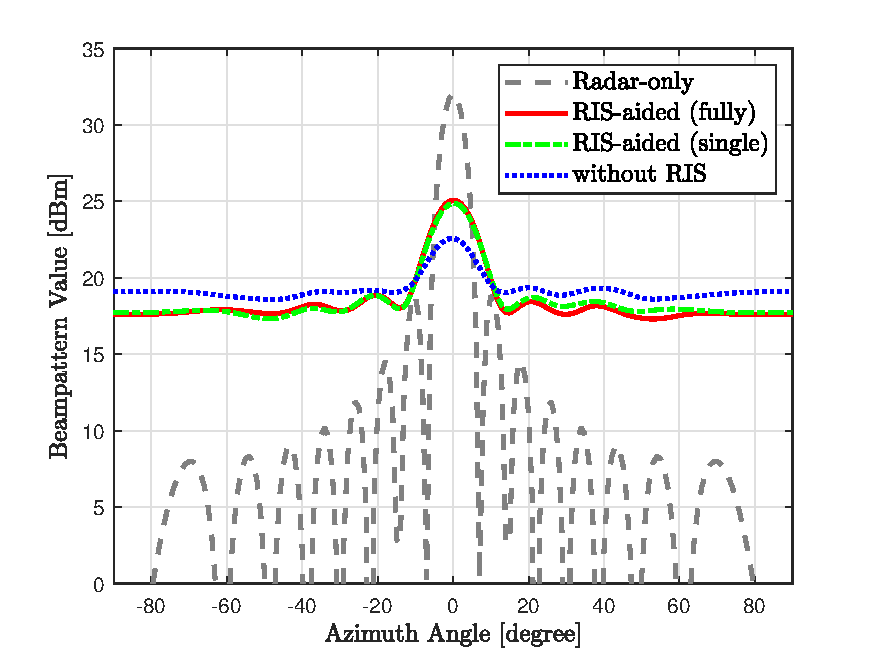
\includegraphics[width=0.95\textwidth]{fig/beampattern_los_single_fully_b}\vspace{2pt}\\
            \small{b) Separated, LOS}
        \end{minipage}  
    \end{minipage}
    \begin{minipage}[c]{0.37\textwidth}
        \vspace{10pt}
        \begin{minipage}[c]{\textwidth}
            \centering
            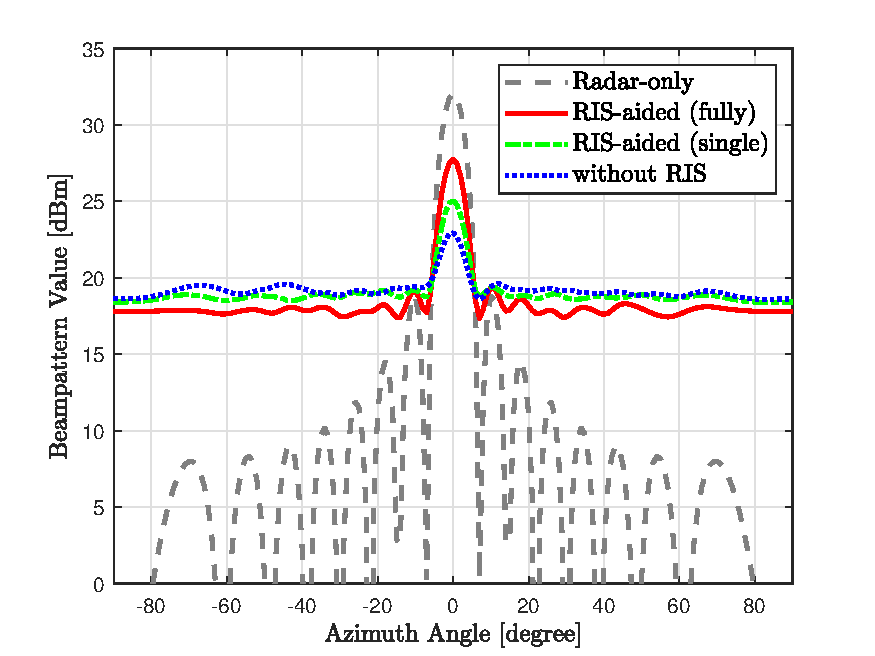
\includegraphics[width=0.95\textwidth]{fig/beampattern_rayleigh_single_fully_d}\vspace{2pt}\\
            \small{c) Shared, Rayleigh}
        \end{minipage}\vspace{10pt}\\
        \begin{minipage}[c]{\textwidth}
            \centering
            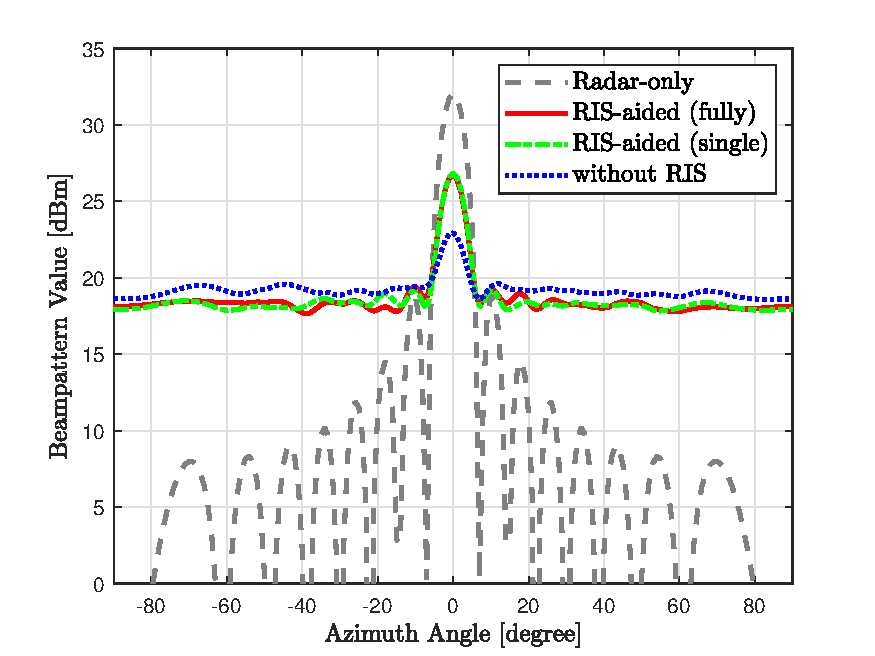
\includegraphics[width=0.95\textwidth]{fig/beampattern_los_single_fully_d}\vspace{2pt}\\
            \small{d) Shared, LOS}
        \end{minipage}  
    \end{minipage}


}


%%% Tradeoff %%%%%%%%%%%%%%%%%%%%%%%%%%%%%%%%%%%%%%%%%%%%%%%%%%%%%%%%%%%%%%%%
\headerbox{Tradeoff}{name=tradoff, column=2,span=1, below=algorithm, bottomaligned = beampattern}{
    \begin{minipage}[c]{\textwidth}
        \vspace{10pt}
        \centering
        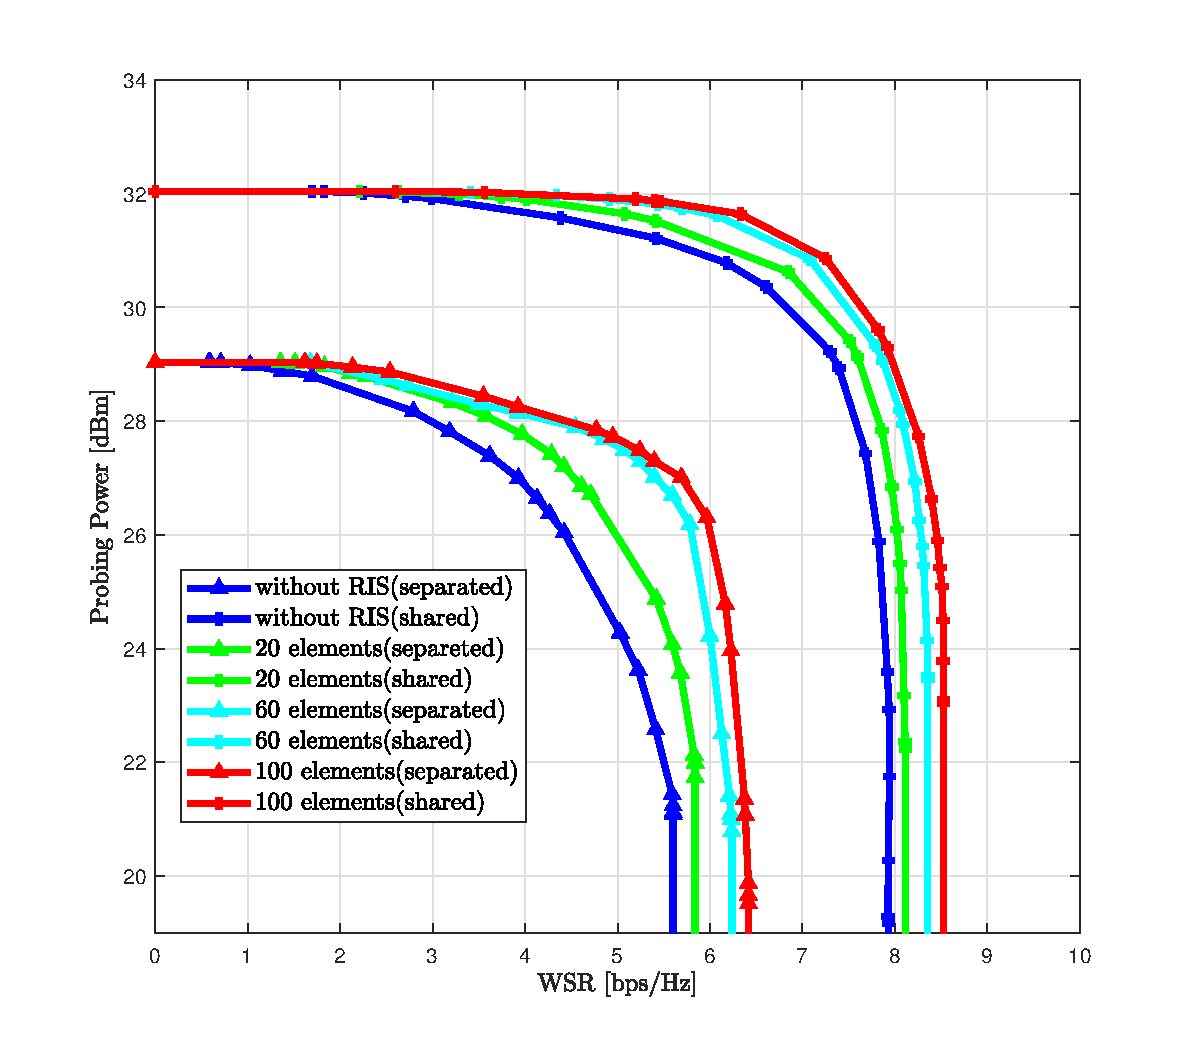
\includegraphics[width=0.95\textwidth]{fig/tradeoff_reflecting_element}\\
        \small{a) Effect of the number of reflecting elements}
    \end{minipage}\\
    \begin{itemize}[leftmargin=1em]
        \vspace{-2pt}\item[$\blacktriangleright$]  With the increase of the number of reflecting elements at RIS, the achievable
        region becomes larger but asymptotically reaches an upper limit.
        \vspace{-2pt}\item[$\blacktriangleright$]  Shared deployment achieves significantly larger achievable region than separated deployment.
    \end{itemize}
    
}

%%% References %%%%%%%%%%%%%%%%%%%%%%%%%%%%%%%%%%%%%%%%%%%%%%%%%%%%%%%%%%%%%%%%
%\headerbox{References}{name=references,column=2,span =1, below=group, bottomaligned=conclusion}{

% make text smaller in this box
%\footnotesize

% Remove the "References":
% http://tex.stackexchange.com/questions/33316/bibtex-with-no-references-title
%\renewcommand\refname{}
%\vspace*{-1.5em}

%\bibliographystyle{ieeetr}
%\bibliography{refs}{}
%}

\end{poster}
\end{document}
